\documentclass{article}
\usepackage[utf8]{inputenc}
%\usepackage[T1]{fontenc}
\usepackage{tikz}
\usepackage{amsthm}
\usepackage{amsmath}
\usepackage{amssymb}
\usepackage{mathtools}
\usepackage{graphicx}
\newtheorem*{definition*}{Definition}
\newtheorem*{property*}{Property}
\newcommand\sbullet[1][.5]{\mathbin{\vcenter{\hbox{\scalebox{#1}{$\bullet$}}}}}
\DeclarePairedDelimiter{\norm}{\lVert}{\rVert}
\DeclarePairedDelimiter{\abs}{|}{|}

\usepackage{hyperref}
\hypersetup{
  colorlinks=true,
  linkcolor=blue,
  filecolor=magenta,      
  urlcolor=cyan,
}



\author{phunc20}
\title{Backprop: A Simple Case}
%\date{21 January, 2022}
%\date{January 22, 2022}
\date{January 21, 2021}

\begin{document}

\maketitle
%\tableofcontents

%\begin{abstract}
%\end{abstract}

\section{Try to Find $\frac{\partial{L}}{\partial{W_1}}$}
Let's try to find a typical gradient, say $\frac{\partial{L}}{\partial{W_1}}$, and hope that
the other gradients could be computed in a similar manner.



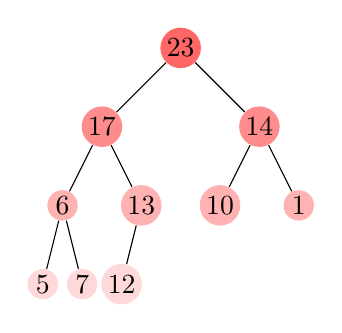
\begin{tikzpicture}[level distance=10mm]
  \tikzstyle{every node}=[fill=red!60,circle,inner sep=1pt]
  \tikzstyle{level 1}=[sibling distance=20mm,
    set style={{every node}+=[fill=red!45]}]
  \tikzstyle{level 2}=[sibling distance=10mm,
    set style={{every node}+=[fill=red!30]}]
  \tikzstyle{level 3}=[sibling distance=5mm,
    set style={{every node}+=[fill=red!15]}]
  \node {23}
    child {node {17}
      child {node {6}
        child {node {5}}
        child {node {7}}
      }
      child {node {13}
        child {node {12}}
        child[fill=none] {edge from parent[draw=none]}
      }
    }
    child {node {14}
      child {node {10}}
      child {node {1}}
    };
\end{tikzpicture}





\end{document}
